\chapter{Data Analysis} \label{DataAnalysis}
This chapter analyzes the results of the 16 users tested. As discussed prior, the group was split into 8 Professionals and 8 Non-musicians and Amateurs. It begins with a validation of findings from past sensorimotor synchronization research and claims mentioned in the SMS expectations section of Chapter 1 (\ref{SMSfindings}).

The results were overall promising, with the haptic modality outperforming audible, as expected, across dynamic beats. Specifically...

\section{SMS Research Confirmations}
Expect as IOI increases, $(SD_{asy})$ increases non linearly

Expect linear increase in NMA as IOI increases for non musicians

Expect non-isochronous tapping to introduce distortions within ITI

Expect positive mean asynchrony when approaching biomechanical limit (<300 ms or 180 bpm)

Expect lower $(SD_{asy})$ for professionals vs non musicians

Expect little to no difference between amatuers and non musicians

Expect percussionists and pianists to have the lowest variability

Expect relatively constant NMA for changing IOI (dynamic tests)


\section{Results}
Overall negative mean asynchrony
- Audible tests
- Haptic tests

\begin{figure}[H]
    \centering
    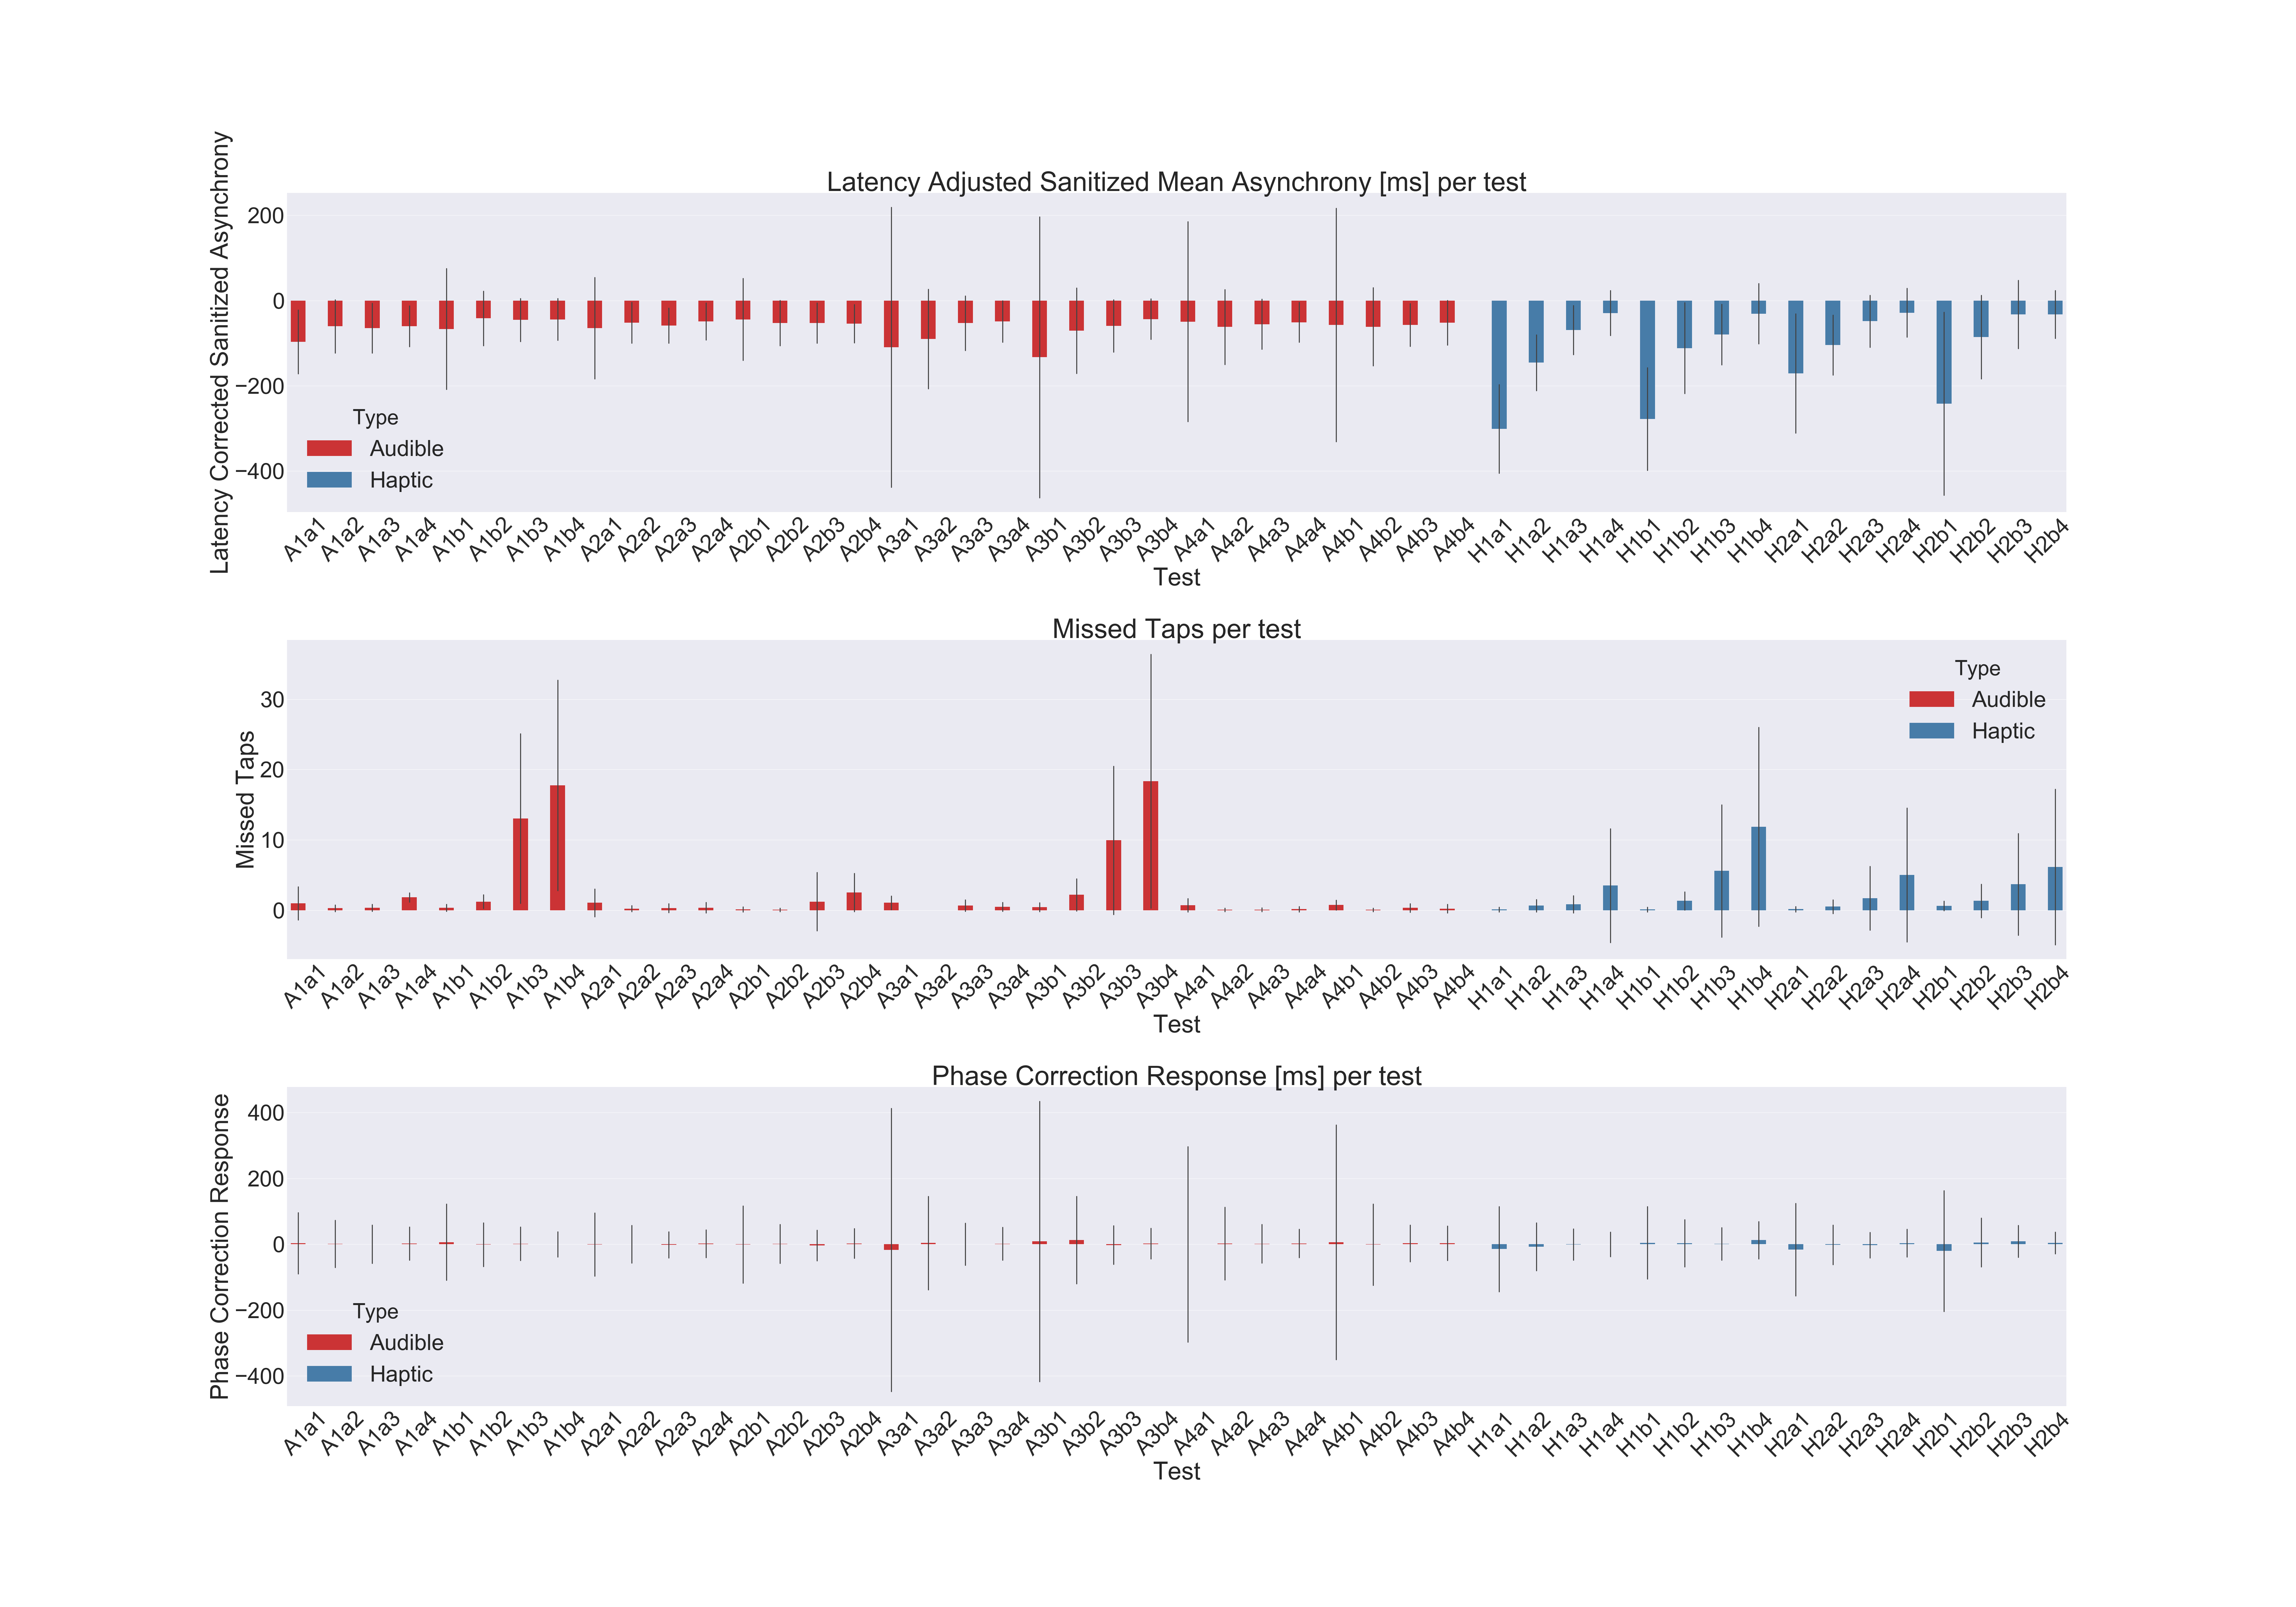
\includegraphics[width=\columnwidth]{AllSummary.png}
    \caption{Overview of all tests across all participants}
    \label{fig:AllSummary}
\end{figure}

Plot normalized stability $(SD_{asy})$ vs IOI

Plot ITI vs IOI

Plot PCR
